\chapter{\label{chap:modeling}Modelagem}
O objetivo deste capítulo é, com base na fundamentação teórica apresentada no
Capítulo \ref{chap:theory} e em uma série de limitações impostas pelo
\textit{framework SpelunkBots}, indicar nossas escolhas de modelagem para
desenvolver os agentes inteligentes jogadores de \textit{Spelunky}.

Na seção \ref{section:spelunkbots-limitations}, apresentamos as limitações
impostas pelo \textit{framework SpelunkBots} que encontramos ao longo do
desenvolvimento deste trabalho. Em seguida, nas seções
\ref{section:modelling-vision} e \ref{section:modelling-outputs}, destacamos as
restrições de visão e ações disponíveis que escolhemos para facilitar o
treinamento dos agentes. Após, na seção \ref{section:modelling-network},
descrevemos as configurações das redes neurais utilizadas. Por fim, nas seções
\ref{section:modelling-genetic} e \ref{section:modelling-fitness}, detalhamos as
configurações utilizadas para o algoritmo genético do \textit{NEAT} e as funções
de aptidão utilizadas para realizar o treinamento dos agentes.


%----------
\section{\label{section:spelunkbots-limitations}Limitações do
\textit{SpelunkBots}}
Uma das partes centrais de nosso trabalho é o uso do \textit{framework}
\textit{SpelunkBots} para realizar a comunicação dos agentes inteligentes com o
jogo \textit{Spelunky}. Contudo, esta ferramenta possui algumas limitações
importantes de serem ressaltadas, pois elas afetam diretamente umas as outras e
causam um impacto significativo de performance de execução:

\begin{description}
	\item[Aceleração de Execução]
		Apesar de a ferramenta disponibilizar um mecanismo para permitir a
		aceleração da execução do jogo (através dos botões \textit{PageUp} e
		\textit{PageDown}), este efeito não pôde ser verificado quando
		realizamos alguns testes iniciais na ferramenta.

	\item[Contagem de Tempo]
		A contagem do tempo de execução de um nível é feito por fora do jogo,
		através de chamadas da função \textit{GetTickCount} do \textit{Windows}.
		Isto resulta em pelo menos dois efeitos colaterais. O primeiro é que se,
		por exemplo, pausarmos a execução do jogo e retormarmos a execução após
		um tempo, este intervalo de tempo será contabilizado como tempo de
		execução. O segundo é que se, por qualquer motivo, o jogo sofrer uma
		queda de desempenho momentânea (mais processamento de CPU, por exemplo),
		a contabilização do tempo continuará igual, o que significa que máquinas
		com capacidade de processamento inferiores não possuem, realisticamente
		falando, o mesmo tempo de execução que máquinas mais potentes.

	\item[Chamadas de DLL]
		Devido às limitações de programação externa oferecidas pelo
		\textit{GameMaker} como, por exemplo, a compatibilidade de chamada de
		funções	externas somente com tipo de retorno \textit{double} e
		\textit{char*}, a ferramenta precisa realizar várias chamadas de
		\textit{DLL} por etapa de execução para atualizar suas variáveis. Isto
		afeta a performance, resultando em um péssimo desempenho e código não
		otimizado.

	\item[Execução com Gráficos]
		Atualmente, é impossível executar a ferramenta sem janela gráfica, o que
		significa que, a cada certo período de tempo, é preciso renderizar o
		jogo. Durante o o treinamento dos agentes, essa função é desnecessária,
		ou seja, gasta-se tempo e capacidade de processamento para uma
		funcionalidade que não é utilizada.

	\item[Sistema Operacional]
		A ferramenta \textit{SpelunkBots} foi desenvolvida somente para a
		plataforma \textit{Windows}, o que significa que, para executá-la em
		outras plataformas (no nosso caso, \textit{Linux}), é preciso utilizar
		programas adicionais para realizar a compilação e execução do jogo. Este
		\textit{overhead} adicional prejudica o desempenho da aplicação.
\end{description}


%----------
\section{\label{section:modelling-vision}Visão do Agente}
Conforme detalhado anteriormente na Seção \ref{section:spelunkbots-information},
É possível receber informações de nodos do mapa, inimigos e objetos durante a
execução do jogo. Como nosso objetivo é tratar somente o domínio de navegação,
estamos interessados apenas nas informações de nodos do mapa. Devido ao sistema
de \textit{fog of war} (Figura \ref{fig:spelunkbots-fow}), não temos acesso
ilimitado às informações do mapa, restringindo-nos apenas a nodos que o jogador
já visualizou.

Contudo, seria inviável utilizar toda a visão disponível por três motivos. O
primeiro motivo é que estamos utilizando uma rede neural com número de entradas
fixa, então não é possível adicionar novos nodos de entrada durante a execução
do programa. O segundo motivo é que utilizar um número de entradas muito grande
resultaria em uma rede com muitas ligações, o que implicaria em uma necessidade
maior de tempo de processamento. O terceiro e último motivo é que, dadas as
limitações da ferramenta \textit{SpelunkBots} apresentadas na seção
\ref{section:spelunkbots-limitations}, identificamos que devemos buscar pela
simplicidade, pois caso contrário a performance dos agentes será afetada.

Outra questão importante é identificar quais são os tipos de nodos que são
interessantes para o domínio da navegação. Nodos como, por exemplo, o altar de
sacrifício, ou armadilhas de flechas não são pertinentes ao problema que
desejamos tratar inicialmente. Já nodos como o chão escorregadio ou a armadilha
de lanças apresentam grandes desafios a serem superados, e é provável que não
seja uma boa ideia considerá-los originalmente.

Optamos, portanto, por limitar a visão do agente em dois aspectos:

\begin{itemize}
	\item \textbf{Região de Visão:} o agente só será capaz de receber
		informações de nodos em sua proximidade, em uma região quadrada ao seu
		redor. A Figura \ref{fig:vision-limitation} ilustra um exemplo de região
		de visão dos agentes.

	\item \textbf{Tipos de Nodo:} limitamos os tipos de nodo que o agente é
		capaz de visualizar, permitindo somente nodos dos tipos: vazio, terreno
		, saída, escada e espinho. Caso o agente visualize qualquer outro tipo
		de nodo durante a execução, ele o interpretará como um nodo do tipo
		terreno. A Figura \ref{fig:vision-nodes} ilustra os nodos que o agente é
		capaz de enxergar.
\end{itemize}

\begin{figure}[htb!]
\centering
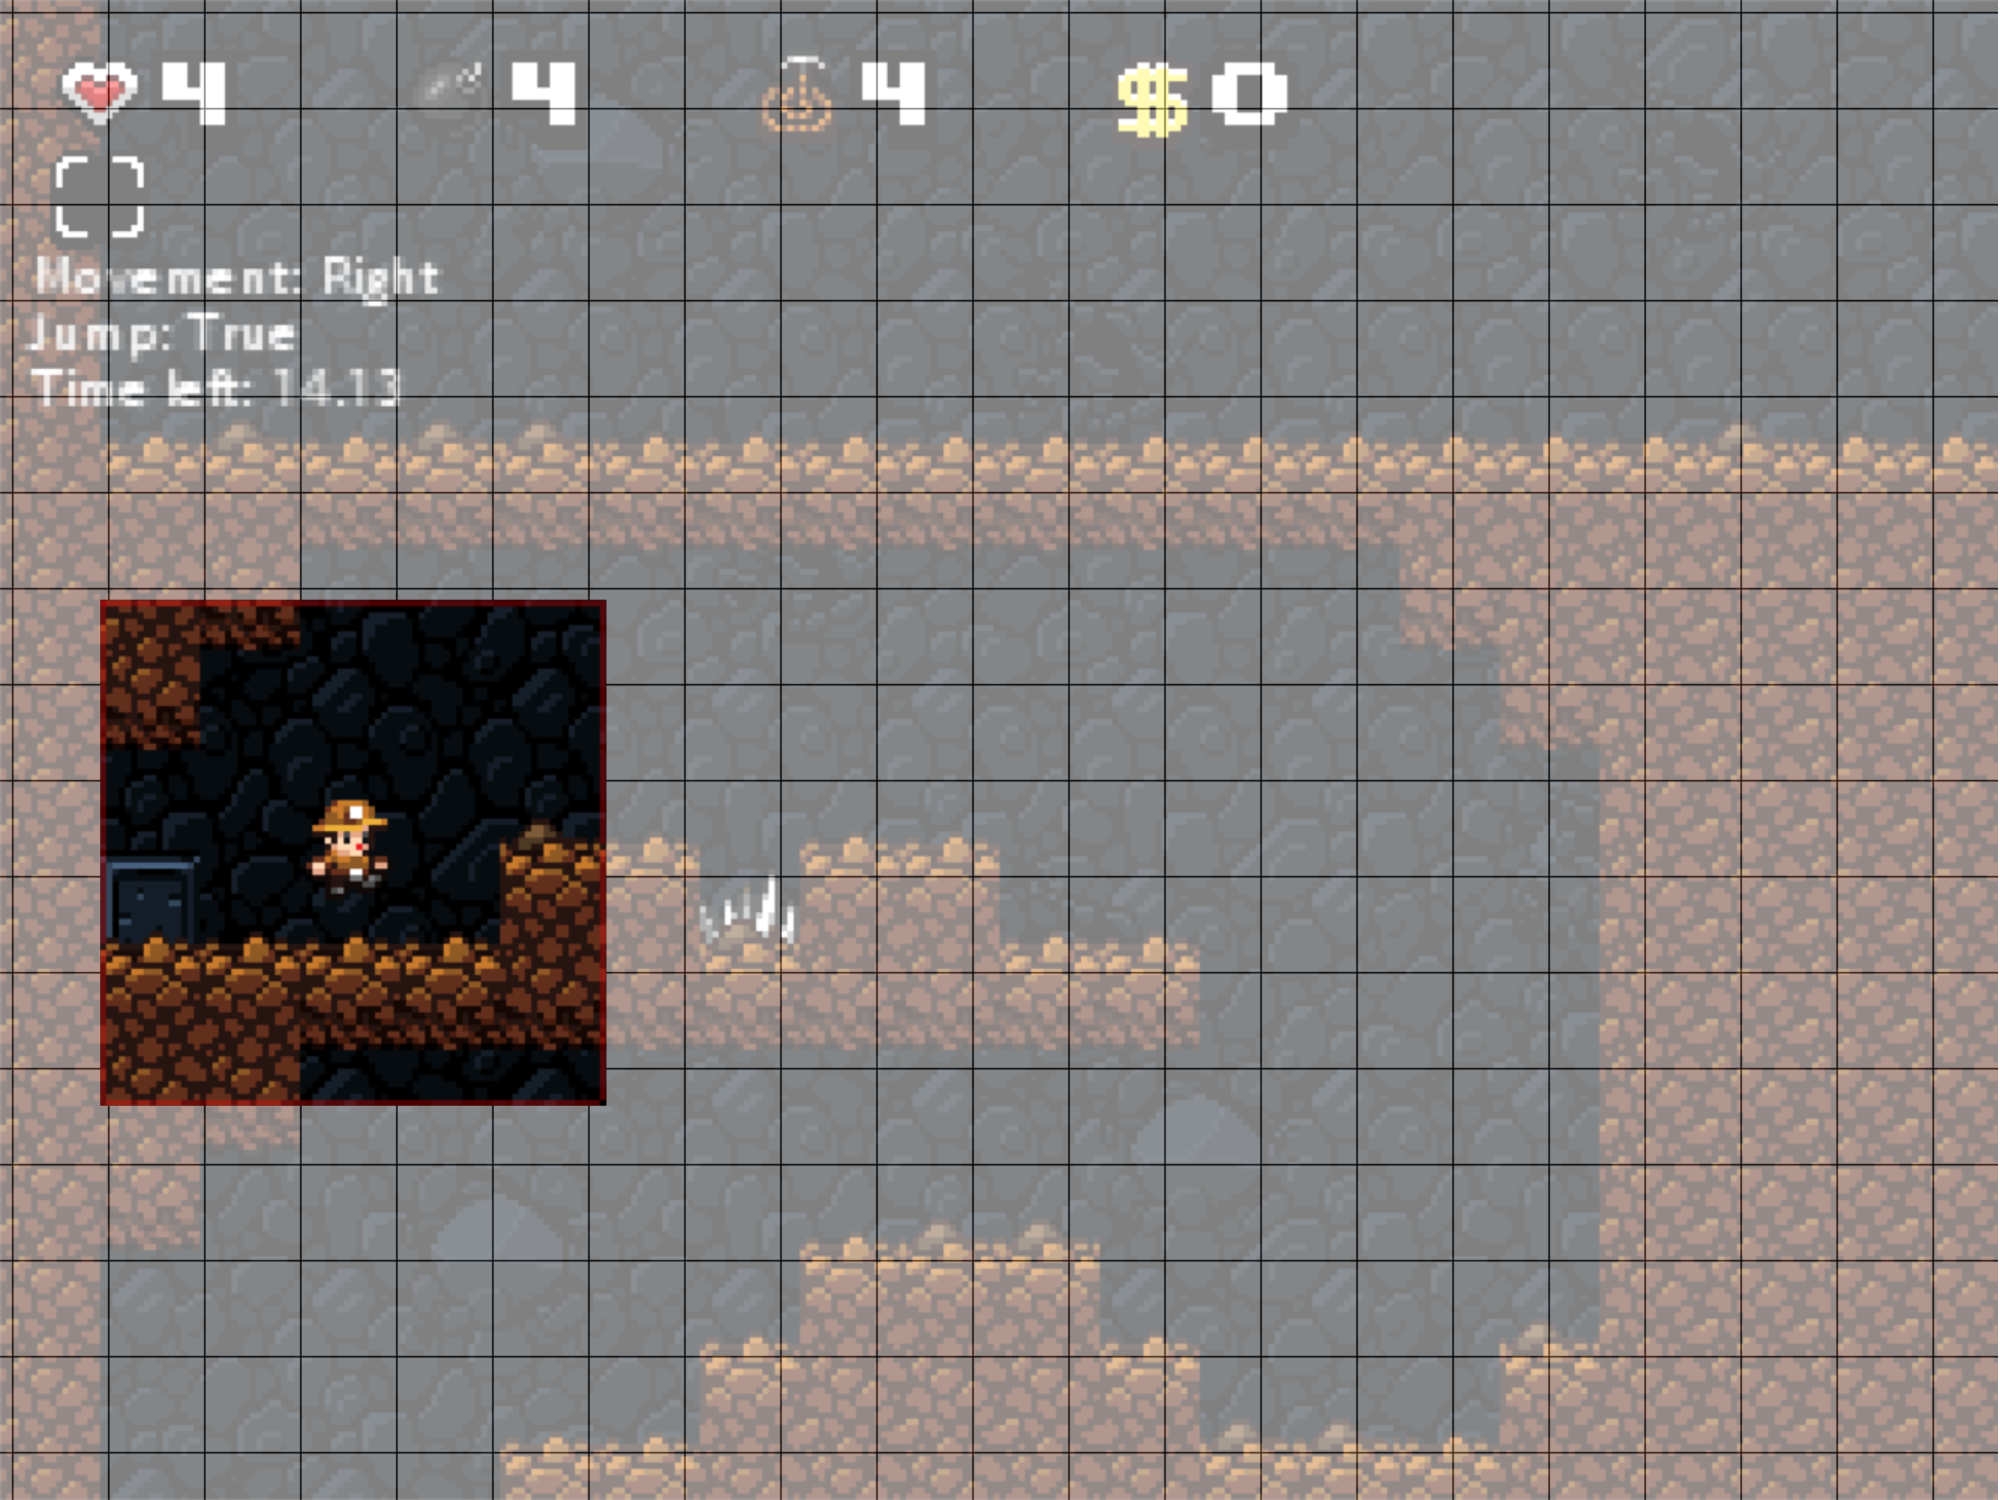
\includegraphics[width=.65\textwidth]{fig/spelunkbots-bot-vision.pdf}
\caption{\label{fig:vision-limitation}Exemplo da visão que um agente jogador de
\textit{Spelunky} tem enquanto está jogando.}
\end{figure}

\begin{figure}[H]
\centering
	\begin{subfigure}[b]{0.15\textwidth}
        
\includegraphics[width=\textwidth]{fig/spelunky-empty.pdf}
		\caption{Vazio.}
	\end{subfigure}
	\begin{subfigure}[b]{0.15\textwidth}
        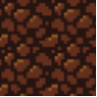
\includegraphics[width=\textwidth]{fig/spelunky-terrain.pdf}
		\caption{Terreno.}
	\end{subfigure}
	\begin{subfigure}[b]{0.15\textwidth}
        
\includegraphics[width=\textwidth]{fig/spelunky-end-door.pdf}
		\caption{Saída.}
	\end{subfigure}
	\begin{subfigure}[b]{0.15\textwidth}
        
\includegraphics[width=\textwidth]{fig/spelunky-stair.pdf}
		\caption{Escada.}
	\end{subfigure}
	\begin{subfigure}[b]{0.15\textwidth}
        
\includegraphics[width=\textwidth]{fig/spelunky-spike.pdf}
		\caption{Espinho}
	\end{subfigure}
	\caption{Exemplos dos nodos que o agente é capaz de enxergar.}
	\label{fig:vision-nodes}
\end{figure}

Não é possível identificar de antemão qual tamanho de visão será o mais adequado
para o agente sem realizar algum tipo de experimentação para realizar uma
validação empírica. Portanto, durante o treinamento dos agentes, realizaremos um
experimento para testar alguns tamanhos de área de visão (seção
\ref{section:experiment-vision}).


%----------
\section{\label{section:modelling-outputs}Ações do Agente}
A ferramenta \textit{SpelunkBots} permite que o agente envie comandos de ação
para o personagem (detalhado na Seção \ref{section:spelunkbots-commands}). Para
tal, o agente deve modificar uma série de variáveis que estão mapeadas para os
botões de ação. Em \textit{Spelunky}, o jogador é capaz de executar um grande
número de ações -- e combinações de ações -- a cada etapa de atualização do
jogo. Algumas delas são influenciadas por itens equipados ou o estado atual do
jogador (no ar, pendurado, etc.), o que significa que o agente deve estar
preparado para lidar com uma gama gigantesca de possibilidades de ações.

Considerar todas as ações disponíveis não é uma boa ideia por dois motivos.
Primeiramente, muitas destas ações não são necessárias para navegar pelo mapa, e
algumas podem inclusive, irônicamente, dificultar a navegação, como colocar
bombas ou cordas, pois criariam mais problemas do que resolveriam (rotas
adicionais, lidar com pontos de vida, etc.). Por fim, como mencionamos na seção
\ref{section:modelling-vision}, devido às limitações do \textit{SpelunkBots}, o
tamanho da rede neural pode influenciar na performance dos bots. Portanto, é
interessante eliminar a possibilidade de execução de todas as ações que não
trarão benefício para a navegação.

Assim, limitamos as ações que os agentes podem executar a \textbf{Movimentação}
(Esquerda e Direita) e \textbf{Pulo}. Caso algum dos cenários de teste
desenvolvidos requira ações adicionais, incluiremos conforme necessidade. Desta
forma, manteremos um controle ainda maior sobre cada caso de teste.


%----------
\section{\label{section:modelling-network}Configurações da Rede Neural}
Todos os agentes realizam a tomada de decisão de quais ações tomar baseados em
uma rede neural. Portanto, é importante detalhar como decidimos configurá-las
para execução. Esta configuração foi baseada em nosso levantamento de material
teórico, localizado no Capítulo \ref{chap:theory}. Existem duas partes
fundamentais de nossas redes neurais que devem ser inspecionadas: os
\textbf{neurônios} e a \textbf{topologia}.

Existem três pontos significativos de configuração dos neurônios da rede neural,
que são os \textbf{intervalos de pesos de conexões}, encarregados de informar
aos neurônios o quao importante é a informação, a \textbf{função de integração},
responsável por unificar os dados que estão entrando no neurônio, e a
\textbf{função de ativação}, cujo papel é processar o resultado da função de
integração. Como estamos utilizando uma biblioteca de \textit{NEAT}, estas
configurações estão pré-estabelecidas, e são as seguintes: o intervalo de
valores de pesos é entre $-8$ e $8$; a função de integração é uma simples
adição; a função de ativação é do tipo sigmóide, mais especificamente, a função
logística, que mantém os valores normalizados no intervalo $[0,1]$:

\begin{equation}
	\label{eq:neat-activation}
	f(x) = \frac{1}{1+e^{-k*m}}
\end{equation}

onde $e$ é o número de \textit{Euler} (2.71828), $k$ é a inclinatura da curva
(4.924273) e $m$ é o valor de soma atual dentro do neurônio.

As especificações de topologia inicial também são determinadas pelo
\textit{NEAT}, conforme vimos na seção \ref{section:neat}. Apear de possuirmos a
opção de incluir recorrência na rede, optamos por deixar a rede o mais simples
possível (sem realimentação), porque este processamento extra poderia levar a um
gargalo de execução, afetando a pontuação dos agentes devido a uma perda de
tempo. Na camada de entrada, colocamos um nodo de \textit{bias} e  fizemos a
conexão dos dados de visão recebidos pelo \textit{SpelunkBots}, conforme citado
na seção \ref{section:modelling-vision}. Ou seja, caso o tamanho do campo de
visão de um agente for de uma área de 5 por 5, a rede teria 25 nodos de visão e
1 nodo de \textit{bias}, totalizando em 26 nodos de entrada. A técnica
\textit{NEAT} também especifica que, inicialmente, não devem existir camadas
escondidas na rede, para que a evolução possa acontecer somente conforme
necessidade. Portanto, nossas redes neurais não possuem, inicialmente, nenhuma
camada escondida. Nas saídas da rede, fizemos o mapeamento, um para um, das
ações que desejamos executar (listadas na seção \ref{section:modelling-outputs}).
Ou seja, se um agente pode executar duas ações, existirão dois nodos de saída na
rede.

Durante o início do desenvolvimento deste trabalho, a ação de movimentação
estava separada em dois nodos, um para esquerda e outro para a direita. Contudo,
como desejávamos diminuir ao máximo o tamanho da rede para diminuir o
processamento necessário, decidimos unir estes dois nodos em um só. Caso o valor
de saída do nodo de movimentação esteja entre $[0,0.4]$, o agente ativará a ação
de caminhar para a esquerda. Se o valor estiver entre $(0.4,0.6)$, o agente não
executará nenhuma ação de movimentação (zona morta). Por fim, caso o valor
esteja entre $[0.6,1]$, o agente executará a ação de caminhar para a direita.

Na primeira etapa de execução, os neurônios da camada de entrada estão ligados,
todos para todos, com os neurônios da camada de saída. Portanto, para calcular o
número inicial de conexões da rede, basta utiliarmos a fórmula:

\begin{equation}
	\label{eq:network-connections}
	C = N_e * N_s
\end{equation}

onde $N_e$ é o número de neurônios na camada de entrada e $N_s$ corresponde ao
número de neurônios na camada de saída. Sem a modificação citada acima, um
neurônio de \textit{bias} e um tamanho de área de visão de 5 por 5, nossa rede
neural possuiria $78$ conexões.  Com esta pequena modificação, o número de
conexões cai para $52$. A diferença parece ser insignificante, mas este é apenas
o número de conexões na primeira etapa de execução. Conforme o algoritmo
executa, mais nodos e conexões surgirão, portanto diminuir o número de conexões
iniciais pode ter um impacto significante com o passar do tempo. A Figura
\ref{fig:modelling-network-example} ilustra uma configuração inicial de rede
neural utilizada neste trabalho.

\begin{figure}[H]
\centering
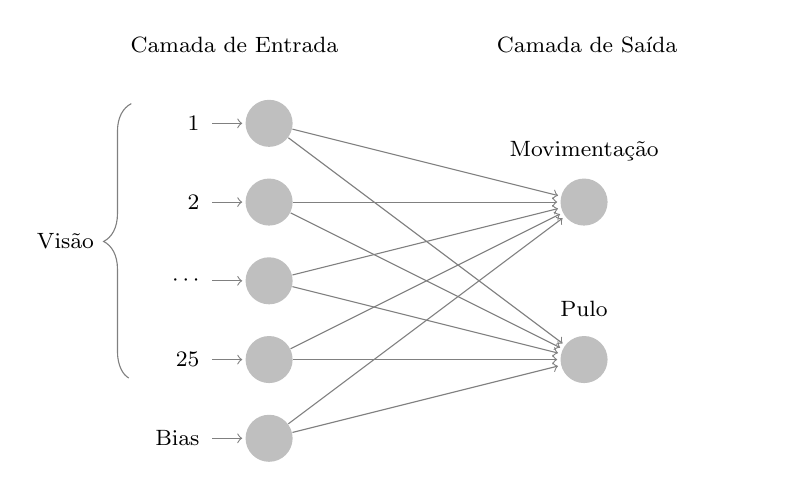
\begin{tikzpicture}[shorten >=1pt,->,draw=black!50, node distance=\layersep]
    \def\layersep{4cm}
    \tikzstyle{every node}=[font=\footnotesize]
    \tikzstyle{every pin edge}=[<-,shorten <=1pt]
    \tikzstyle{neuron}=[circle,fill=black!25,minimum size=17pt,inner sep=0pt]
    \tikzstyle{input neuron}=[neuron, fill=gray!50];
    \tikzstyle{output neuron}=[neuron, fill=gray!50];
    \tikzstyle{hidden neuron}=[neuron, fill=gray!50];
    \tikzstyle{annot} = [text width=10em]

    \node[input neuron, pin=left:1]        (I-0) at (0, 0)  {};
    \node[input neuron, pin=left:2]        (I-1) at (0, -1) {};
    \node[input neuron, pin=left:$\cdots$] (I-2) at (0, -2) {};
    \node[input neuron, pin=left:25]       (I-3) at (0, -3) {};
    \node[input neuron, pin=left:Bias]     (I-4) at (0, -4) {};

    \draw[decoration={brace,mirror,amplitude=10pt},decorate, style={-}]
      (-1.75,0.25) -- node[midway, left=10pt] {Visão} (-1.75, -3.25);

    \node at (\layersep, -0.35) {Movimentação};
    \node[hidden neuron] (O-0) at (\layersep, -1) {};
    \node at (\layersep, -2.35) {Pulo};
    \node[hidden neuron] (O-1) at (\layersep, -3) {};

    \foreach \source in {0,...,4}
        \foreach \dest in {0,...,1}
            \path (I-\source) edge (O-\dest);
    \node[annot] at (0, 1) {Camada de Entrada};
    \node[annot] at (4.65cm, 1) {Camada de Saída};
\end{tikzpicture}
\caption {\label{fig:modelling-network-example}Exemplo de configuração de rede
	neural inicial com campo de visão 5 por 5.}
\end{figure}

Conforme mencionado na seção \ref{section:modelling-outputs}, adicionaremos
neurônios na camada de saída conforme necessidade, ou seja, caso algum cenário
de teste exija do agente alguma ação a mais, esta ação será inserida na rede
inicial.

\subsection{\label{section:obstacle-input}Detecção de Obstáculos}
Durante a execução dos experimentos, listados no Capítulo
\ref{chap:experimentation-and-results}, pensamos em uma maneira de auxiliar o
agente a aprender mais rapidamente a superar alguns níveis. Esta ideia consistia
em informar para o agente, de alguma maneira, que ele havia esbarrado em uma
parede que não seria capaz de transpor com as ações disponíveis (movimentação e
pulo). Como o agente não consegue transpor uma parede com mais de 2 
\textit{tiles} de altura (exemplo ilustrado pela Figura \ref{fig:obstacle}),
qualquer parede com 3 ou mais blocos de altura seria considerada um obstáculo
intransponível. Assim, esperávamos que o agente, ao identificar tal obstáculo,
alterasse de alguma maneira sua rota, para que houvesse uma ``desubstruição''.

\begin{figure}[htb!]
\centering
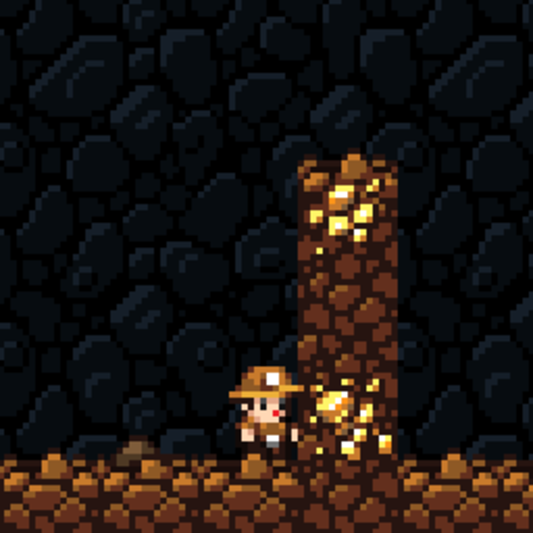
\includegraphics[width=.2\textwidth]{fig/obstacle.pdf}
\caption{\label{fig:obstacle}Exemplo de obstáculo intransponível.}
\end{figure}

Uma maneira de transferir este conhecimento para o agente é através de sua rede
neural. Como todos os neurônios da camada de entrada estão, inicialmente,
conectados à camada de saída, esta informação seria transportada para o neurônio
de movimentação, ajustando seu valor de acordo com a presença de um obstáculo.
Desta forma, optamos por incluir, em alguns cenários de teste, um neurônio
adicional na camada de entrada que seria responsável por informar ao agente
sobre a existência de um obstáculo intransponível na sua frente. Esta
configuração inicial de rede é ilustrada pela Figura \ref{fig:network-obstacle}.

\begin{figure}[H]
\centering
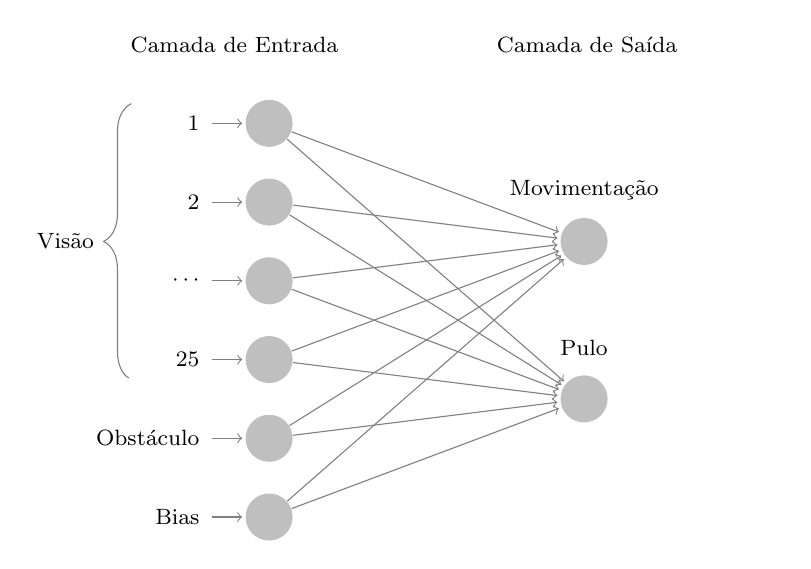
\begin{tikzpicture}[shorten >=1pt,->,draw=black!50, node distance=\layersep]
    \def\layersep{4cm}
    \tikzstyle{every node}=[font=\footnotesize]
    \tikzstyle{every pin edge}=[<-,shorten <=1pt]
    \tikzstyle{neuron}=[circle,fill=black!25,minimum size=17pt,inner sep=0pt]
    \tikzstyle{input neuron}=[neuron, fill=gray!50];
    \tikzstyle{output neuron}=[neuron, fill=gray!50];
    \tikzstyle{hidden neuron}=[neuron, fill=gray!50];
    \tikzstyle{annot} = [text width=10em]

    \node[input neuron, pin=left:1]         (I-0) at (0, 0)  {};
    \node[input neuron, pin=left:2]         (I-1) at (0, -1) {};
    \node[input neuron, pin=left:$\cdots$]  (I-2) at (0, -2) {};
    \node[input neuron, pin=left:25]        (I-3) at (0, -3) {};
    \node[input neuron, pin=left:Obstáculo]      (I-4) at (0, -4) {};
    \node[input neuron, pin=left:Bias] (I-5) at (0, -5) {};

    \draw[decoration={brace,mirror,amplitude=10pt},decorate, style={-}]
      (-1.75,0.25) -- node[midway, left=10pt] {Visão} (-1.75, -3.25);

    \node at (\layersep, -0.85) {Movimentação};
    \node[hidden neuron] (O-0) at (\layersep, -1.5) {};
    \node at (\layersep, -2.85) {Pulo};
    \node[hidden neuron] (O-1) at (\layersep, -3.5) {};

    \foreach \source in {0,...,5}
        \foreach \dest in {0,...,1}
            \path (I-\source) edge (O-\dest);
    \node[annot] at (0, 1) {Camada de Entrada};
    \node[annot] at (4.65cm, 1) {Camada de Saída};
\end{tikzpicture}
\caption {\label{fig:network-obstacle}Configuração da rede neural com
a entrada de obstáculo.}
\end{figure}

Inicialmente, este neurônio podia ter dois valores distintos: $0$ para passagem
livre e $1$ para obstrução. A Figura \ref{fig:obstacle-input-wrong} ilustra a
configuração de valores de acordo com a presença de obstáculo. Contudo, esta
informação não era suficiente para ajudar o agente porque, quando esbarrava em
uma parede, o valor do neurônio era alterado para $1$ mas, logo em seguida,
quando o agente mudava de direção, o valor retornava para $0$. Isto fazia com
que o agente permanecesse ``travado'' na mesma posição.

\begin{figure}[H]
\centering
	\begin{subfigure}[b]{0.2\textwidth}
        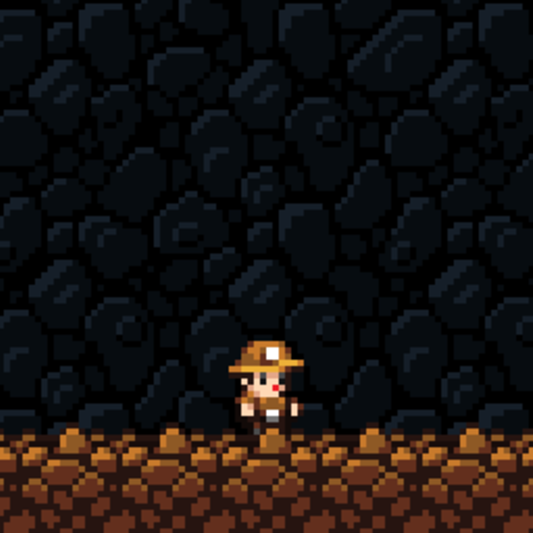
\includegraphics[width=\textwidth]{fig/obstacle-3.pdf}
        \caption{Livre: \textit{0}.}
	\end{subfigure}
	\begin{subfigure}[b]{0.2\textwidth}
        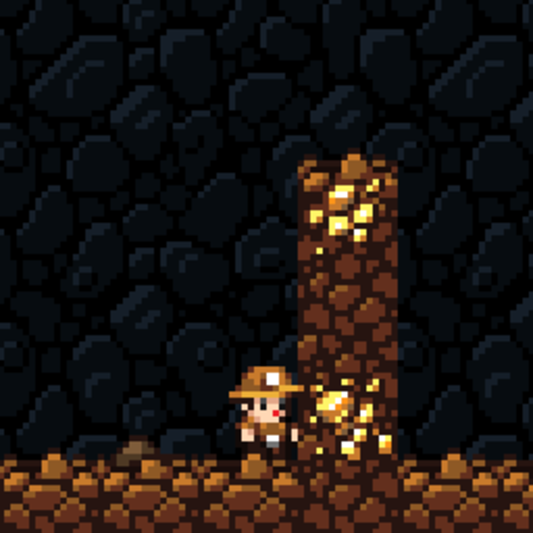
\includegraphics[width=\textwidth]{fig/obstacle.pdf}
        \caption{Obstrução: \textit{1}.}
	\end{subfigure}
    \caption{Configuração de valores de acordo com a presença de obstáculo.}
	\label{fig:obstacle-input-wrong}
\end{figure}

Com esta informação em mente, decidimos trabalhar com a informação de obstáculo
de uma maneira diferente. Agora, existem três possíveis configurações,
ilustradas pela Figura \ref{fig:obstacle-input-correct}:

\begin{description}
	\item[Início]
		No momento inicial de execução, o valor do neurônio de obstáculo será
		$0$. Assim, o agente não será tendencioso em relação a em qual direção
		navegar inicialmente.

	\item[Obstáculo à Esquerda]
		Se o agente estiver caminhando para a esquerda e encontrar um obstáculo,
		o valor do neurônio de obstáculo será alterado para $1$ e permanecerá
		com este valor até que o agente encontre um obstáculo à direita.

	\item[Obstáculo à Direita]
		Se o agente estiver caminhando para a direita e encontrar um obstáculo,
		o valor do neurônio de obstáculo será alterado para $-1$. e permanecerá
		com este valor até que o agente encontre um obstáculo à esquerda.
\end{description}

\begin{figure}[H]
\centering
	\begin{subfigure}[b]{0.2\textwidth}
        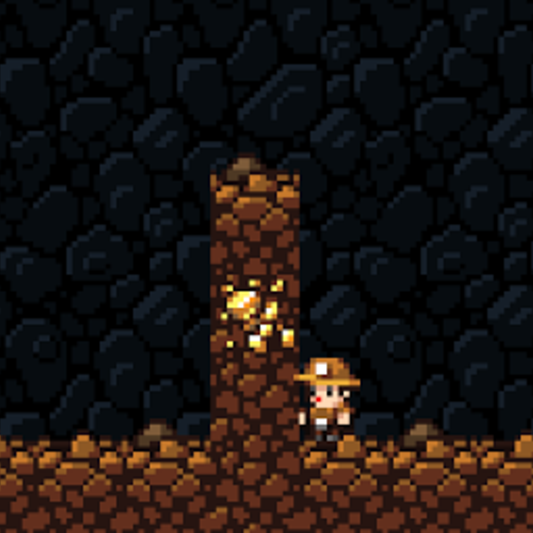
\includegraphics[width=\textwidth]{fig/obstacle-2.pdf}
        \caption{Esquerda: \textit{1}.}
	\end{subfigure}
	\begin{subfigure}[b]{0.2\textwidth}
        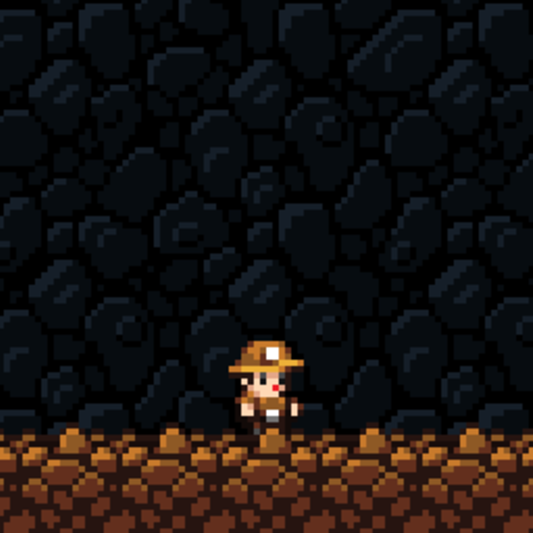
\includegraphics[width=\textwidth]{fig/obstacle-3.pdf}
        \caption{Livre: \textit{0}.}
	\end{subfigure}
	\begin{subfigure}[b]{0.2\textwidth}
        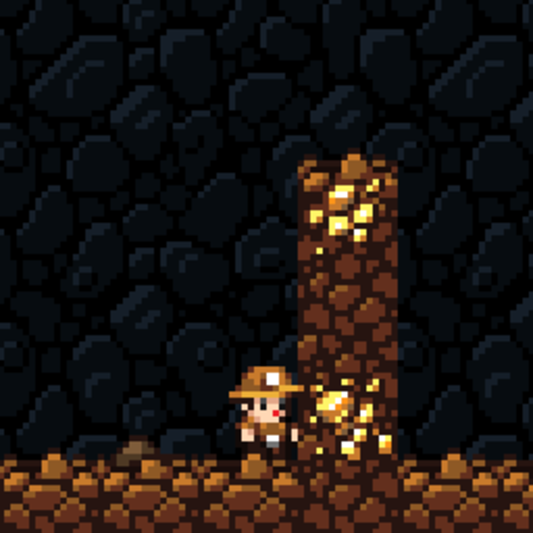
\includegraphics[width=\textwidth]{fig/obstacle.pdf}
        \caption{Direita: \textit{-1}.}
	\end{subfigure}
    \caption{Possíveis configurações de obstáculo.}
	\label{fig:obstacle-input-correct}
\end{figure}

Escolhemos estes valores pelo seguinte motivo: o neurônio de saída de
movimentação decide para qual direção o agente irá caminhar baseado em
intervalos de valor. Caso o valor caia no intervalo de valores mais a esquerda
(até $0.4$), o agente se deslocará para a esquerda. Caso o valor caia no
intervalo de valores mais a direita (de $0.6$ em diante), o agente se deslocará
para a direita. Se o agente estiver caminhando para a esquerda e encontrar um
obstáculo, o valor $1$ do neurônio de obstáculo elevará o valor de saída de
movimentação, forçando-o para um intervalo mais à direita. Do mesmo modo, caso o
agente esteja caminhando para a direita e encontrar um obstáculo, o valor $-1$
reduzirá o valor de saída de movimentação, empurrando-o para um intervalo mais à
esquerda.

Para testar se este neurônio adicional acelerava o aprendizado dos agentes,
preparamos um experimento (seção \ref{section:obstacle-experiment}) com e sem
este neurônio para identificar seu impacto.

%----------
\section{\label{section:modelling-genetic}Configurações do Algoritmo Genético}
A técnica \textit{NEAT}, de acordo com a literatura explorada na seção
\ref{section:neat}, se baseia na neuroevolução para treinar as redes neurais
artificiais. Como ela evolui tanto os pesos das conexões quanto a topologia da
rede, as redes neurais são classificadas como \textit{TWEANNs}. O algoritmo
evolutivo do \textit{NEAT} é muito promissor pois resolve três problemas
extremamente comuns da neuroevolução: a permutação, a proteção da inovação e
população inicial. Listamos, a seguir, as características definidas como mais
importantes de um algoritmo genético, definido em
\ref{section:evolutionary-algorithms}, e como a técnica os resolve:

\begin{description}
	\item[Representação]
		A representação é feita de maneira direta, de acordo com a Figura
		\ref{fig:neat-encoding-example}.

	\item[Função de Aptidão]
		Esta função não é fornecida pelo \textit{NEAT} pois depende do domínio
		do problema. Portanto, deve ser disponibilizada por nós para o
		algoritmo. As descrições das funções de aptidão que desenvolvemos estão
		localizadas na seção \ref{section:modelling-fitness}.

	\item[População]
		O tamanho da população deve ser grande o suficiente para permitir que a
		especiação ocorra e que haja diferenciação genética suficiente entre os
		organismos. Contudo, devido à incapacidade de acelerar a execução do
		\textit{SpelunkBots}, o tamanho da população não pode ser muito elevado,
		pois se não nossos testes levariam tempo demais para concluir. Portanto,
		escolhemos um número de população de \textbf{100} organismos.

	\item[Seleção de Pais] A seleção de pais no \textit{NEAT} é feita de forma
		aleatória. Ou seja, a cada iteração, o algoritmo seleciona um ou dois
		pais para fazer mutações ou cruzamentos, respectivamente.

	\item[Variação] As probabilidades de realizar mutações e cruzamentos na
		biblioteca escolhida (detalhada na seção \ref{section:neat-details}) são
		definidas através de um arquivo externo que mapeia uma característica
		para uma probabilidade de acontecimento. As principais características
		que modificamos foram:
		\begin{itemize}
				\item força de mutação de pesos: $2.5$
				\item probabilidade de mutação de peso: $90\%$
				\item probabilidade de adição de nodo: $3\%$
				\item probabilidade de adição de conexão: $5\%$
				\item tamanho da população: $100$
		\end{itemize}

	\item[Seleção de Sobreviventes]
		A cada iteração, a geração anterior é substituida completamente por uma
		geração nova, baseada na mutação e cruzamento dos organismos anteriores.
		Para criar os novos organismos, o algoritmo organiza as espécies por
		ordem de maior aptidão e, então, distribui um pedaço da população para
		cada uma.

\end{description}

Também selecionamos os valores dos coeficientes de similaridade entre
organismos, integrantes da fórmula \ref{eq:neat-species}:

\begin{itemize}
	\item \textbf{$c_1$ (excess genes):} 1
	\item \textbf{$c_2$ (dijoint genes):} 1
	\item \textbf{$c_3$ (matching genes):} 0.4
\end{itemize}

O valor máximo estipulado para dois organismos pertencerem a mesma espécie,
calculado através da Equação \ref{eq:neat-species}, é de $\delta = 3$.

Para inicializar as redes neurais, o algoritmo conecta todos os neurônios da
camada de entrada com todos os neurônios da camada de saída e cada ligação
possui um peso inicial aleatório. A condição de parada do algoritmo varia de
acordo com o cenário de teste executado, mas sempre será estabelecido um número
máximo de iterações e um tempo máximo de teste.


%----------
\section{\label{section:modelling-fitness}Funções de Aptidão}
A tarefa de criar uma função de aptidão é uma das partes mais difíceis da
aplicação de um algoritmo genético para resolver um problema computacional. Isto
porque o desenvolvedor deve selecionar e experimentar com características do
domínio para encontrar parâmetros que mapeiem corretamente os requisitos que
deseja que seus agentes alcancem dentro do domínio. Se a função não mapear
eficientemente os objetivos desejados, é possível que o algoritmo genético tenha
dificuldades de convergir ou até mesmo convirja para uma solução inapropriada.

Poderiamos definir, por exemplo, uma função de aptidão de maneira extremamente
simplista: se o agente vencer, receberá um valor de aptidão de $1$; caso
contrário, receberá $0$. É possível que esta função funcione eventualmente mas,
dada a complexidade do cenário trabalhado, isto é extremamente improvável. Além
disso, somente o sucesso e o fracasso estão mapeados. Logo, não existe uma
maneira quantitativa de o algoritmo evolutivo identificar resultados
intermediários bons e ruins (retardando o aprendizado), além de ser impossível
identificar quais agentes, entre os bem-sucedidos, são mais eficientes.

Por conseguinte, devemos buscar características do domínio que auxiliem o
algoritmo evolutivo a acelerar o processo de aprendizado. Ao analisarmos o
domínio de navegação e as características de \textit{Spelunky}, identificamos
que nossas funções de aptidão deveriam se basear em duas características
fundamentais: \textbf{distância percorrida} e \textbf{tempo para conclusão}. O
raciocínio por trás da seleção destes parâmetros é simples: se o agente cobrir
uma quantidade maior de terreno, é provável que encontre, eventualmente, a
saída; paralelamente, quanto mais rápido o fizer, mais eficiente o agente será.

É interessante normalizar os valores obtidos de distância e tempo para que
possamos efetuar um balanceamento de importância destes parâmetros. Portanto,
devemos encontrar uma maneira de calculá-los fazendo com que fiquem dentro de
uma determinada região de valores. Um dos requisitos do algoritmo \textit{NEAT}
é que \textbf{os valores de aptidão devem ser positivos}, portanto optamos por
normalizá-los entre o intervalo $[0, 1]$.

\subsection{Distância Percorrida}
Ao iniciar um nível, o personagem é colocado na porta de entrada e deve navegar
pelo mapa e chegar na porta de saída. Um possível cálculo de distância
percorrida é a distância entre a posição final do jogador comparada com a
posição da porta de saída. Contudo, devido ao sistema de \textit{fog of war} do
\textit{SpelunkBots} (ilustrado na Figura \ref{fig:spelunkbots-fow}), não
sabemos qual é a localização exata da porta de saída, a não ser que a
visualizemos durante a execução. Além disso, caso nos baseássemos na distância
do jogador até a porta, nossos agentes obteriam uma vantagem significativa sobre
jogadores humanos, pois mesmo ao ser derrotado, é possível que um humano jamais
saiba a localização exata da porta de saída do mapa que acabou de tentar
superar. Portanto, utilizaremos como \textbf{valor base} a distância entre a
\textbf{posição final do jogador} e a \textbf{posição da porta de entrada}. Este
cálculo de distância se baseará na \textbf{Distância de Manhattan}:

\begin{equation}
	\label{eq:manhattan-distance}
	MD(p_1,p_2) = |p_1.x - p_2.x| + |p_1.y - p_2.y|
\end{equation}

onde $p_1$ e $p_2$ representam as coordenadas $(x,y)$ da porta de entrada e do
jogador, respectivamente. 

Para calcular o parâmetro de distância percorrida de forma normalizada, devemos
encontrar uma forma de estipular um valor máximo aproximado de distância que o
agente pode percorrer. Para tal, nos baseamos nas seguintes características
físicas que todo nível de \textit{Spelunky} apresenta:

\begin{itemize}
	\item os mapas sempre possuem um tamanho fixo de 42 por 34, mas o tamanho de
		área navegável é de 40 por 32 (existe uma borda indestrutível ao redor
		da região do mapa).
	\item o jogador sempre inicia no topo do mapa e a saída sempre se encontra
		na parte inferior do mapa.
\end{itemize}

No pior dos casos, a porta de entrada do mapa estaria localizada na posição
$(1,1)$ e a saída na posição $(40,32)$. Sabendo que o jogador sempre iniciará na
posição da porta de entrada do nível e utilizando a fórmula para distância de
Manhattan, obtemos $D_{max} = 70$, que corresponde ao máximo de distância que o
jogador deverá percorrer.

Agora, com os valores de base e máximo estipulados, é possível utilizar a
seguinte fórmula para calular a aptidão de distância percorrida, normalizada
entre o intervalo $[0,1]$:

\begin{equation}
	\label{eq:distance-fitness}
	D_{n}(p_{1},p_{2}) = MD(p_{1},p_{2}) / D_{max}
\end{equation}

onde $p_1$ e $p_2$ representam as coordenadas $(x,y)$ da porta de entrada e do
jogador, respectivamente. 

\subsection{Tempo para Conclusão}
A ferramenta \textit{SpelunkBots} nos permite estabelecer um tempo máximo de
teste para uma execução ($T_{max}$), bem como detectar o tempo total utilizado
pelo agente durante o teste ($T_{elapsed}$). Com estas duas informações em mãos,
é simples de calcular uma aptião de tempo normalizada entre o intervalo $[0,1]$
através da seguinte fórmula:

\begin{equation}
	\label{eq:time-fitness-wrong}
	T_{n} = (T_{max} - T_{elapsed}) / T_{max}
\end{equation}

Contudo, calcular desta forma a aptidão do parâmetro de tempo resultaria em uma
anomalia indesejada: todos os agentes, independente do resultado da execução,
seriam recompensados (ou penalizados) com uma função de aptidão de tempo igual.
Destacamos, a seguir, alguns dos resultados específicos que encontramos ao
experimentar com este cálculo simples:

\begin{itemize}
	\item Os agentes descobriram que deveriam se matar o mais rápido possível,
		pois assim gastariam pouco tempo durante o teste e sua aptidão de tempo
		seria elevada.

	\item Os agentes que estavam explorando ativamente quando o tempo se
		esgotava eram penalizados da mesma forma que os agentes que morriam, que
		ficavam ociosos e que perambulavam por uma pequena área (não obtendo
		nenhum progresso real).

	\item Todos os agentes que não fossem bem-sucedidos receberiam a mesma
		penalidade: o valor mínimo da função de aptidão de tempo ($0$). Isto
		retarda o processo de aprendizado dos agentes, pois eles só poderão
		depender do parâmetro de distância percorrida para detectar seu
		progresso.
\end{itemize}

Analisando mais à fundo estes resultados, fica claro que existe uma falha na
concepção da função de aptidão de tempo: ela não limita suficientemente o
agente. Na verdade, o agente está fazendo exatamente aquilo que a função de
aptidão de tempo o pede, como fica evidenciado no primeiro resultado citado.
Portanto, decidimos criar um conjunto de regras para a função de aptidão de
tempo, baseada no resultado final da execução:

\begin{description}
	\item[Vitória]
		O agente atingiu a porta de saída. Neste caso sua aptidão de tempo deve
		ser relativa a quanto tempo levou até atingir a porta de saída. Logo,
		utilizamos a fórmula padrão de aptidão de tempo, ilustrada na Equação
		\ref{eq:time-fitness-wrong}.

	\item[Exploração]
		O agente estava explorando ativamente quando o tempo se esgotou. É
		possível que, dado mais tempo, o agente seja capaz de ser bem-sucedido.
		Neste caso, o valor de aptidão de tempo do agente será $0.01$, ou $1\%$
		de $T_{max}$.

	\item[Ocioso]
		O agente estava ocioso por muito tempo. É extremamente provável que
		nunca mais voltasse a se mexer. Neste caso, o valor de aptidão de tempo
		do agente será $0.001$, ou $0.1\%$ de $T_{max}$.

	\item[Repetição de Estados]
		O agente estava explorando apenas uma pequena área do mapa, repetindo
		excessivamente posições que já havia visitado antes. É extremamente
		provável que permaneca desta forma até o fim da execução. Neste caso, o
		valor de aptidão de tempo do agente será $0.001$, ou $0.1\%$ de
		$T_{max}$.


	\item[Morte]
		O agente se matou em um espinho (única forma de se matar atualmente em
		nossos cenários de teste), o que, evidentemente, é um resultado ruim.
		Neste caso, o valor de aptidão de tempo do agente será $0.001$, ou
		$0.1\%$ de $T_{max}$.
\end{description}


\subsection{Fórmulas Escolhidas}
Com os parâmetros de aptidão selecionados, o próximo passo é identificar uma
forma de combiná-los em uma fórmula única de aptidão. Esta parte também é
experimentativa, portanto, escolhemos algumas fórmulas candidatas: \textbf{média
aritmética}, \textbf{média ponderada} e \textbf{média harmônica}. Optamos por
realizar uma média entre os valores porque, apesar de não ser um requisito,
queremos continuar com os valores de aptidão normalizados.

A média aritmética, representada pela Equação \ref{eq:fitness-mean}, é a forma
mais simples de combinarmos os dois parâmetros escolhidos, pois ambos terão a
mesma importância. É possível que o algoritmo evolutivo possua informações
suficientes através desta fórmula.

\begin{equation}
	\label{eq:fitness-mean}
	M_{a} = \frac{D_{n} + T_{n}}{2}
\end{equation}

Já a média aritmética ponderada, representada pela Equação
\ref{eq:fitness-weighted-mean}, busca combinar os parâmetros priorizando de
forma diferente cada parâmetro de aptidão.  Aqui, queremos enfatizar a
importância da navegação, portanto seu peso será maior que o do tempo
necessário. Os valores de peso devem ser entre 0 e 1 e sua soma deve resultar 1.
Os pesos selecionados para distância ($W_{d}$) e tempo ($W_{t}$) serão de
\textbf{0.6} e \textbf{0.4}, respectivamente.

\begin{equation}
	\label{eq:fitness-weighted-mean}
	M_{w} = W_{d}*D_{n} + W_{t}*T_{n}
\end{equation}

Por fim, a média harmônica, representada pela Equação
\ref{eq:fitness-harmonic-mean}, busca combinar os parâmetros enquanto tende a
diminuir o valor da média obtida caso a diferença entre os valores seja muito
elevada. Neste caso, queremos identificar se os melhores resultados de aptidão
ocorrem quando existe um balanceamento entre os parâmetros de distância e tempo.
Caso haja um desbalanceamento, a função tenderá a diminuir a aptidão total dos
agentes.

\begin{equation}
	\label{eq:fitness-harmonic-mean}
	M_{h} = \frac{2}{\frac{1}{D_{n}} + \frac{1}{T_{n}}}
\end{equation}

A escolha de como combinar valores de aptidão baseados em mais de um parâmetro
também é experimentativa. Por isso, executamos testes com todas as funções aqui
citadas para analisar os resultados obtidos com cada uma delas. Tais testes
estão localizados na seção \ref{section:fitness-experiment}.
